\documentclass[11pt]{article}

\usepackage[sexy]{evan} % Evan Chen style
\usepackage{amsmath,amssymb}
\usepackage{array}
\usepackage{caption}
\usepackage{graphicx}
\usepackage{tikz}
\usetikzlibrary{trees}

\fancyhead[L]{}

\title{Sentential Logic -- Chapter 1}
\author{}
\date{}

\begin{document}
\maketitle

%%%%%%%%%%%%%%%%%%%%%%%%%%%%%%%%%%%%%%%%%%%%%%%%%%%%
\section{Informal Remarks on Formal Languages}
%%%%%%%%%%%%%%%%%%%%%%%%%%%%%%%%%%%%%%%%%%%%%%%%%%%%

\begin{remark}[Mini-lesson 1.0.1: Why formal languages?]
We want a symbolic language into which we can translate English sentences.
Unlike natural languages (English, Chinese, \dots), a formal language has
precise formation rules and avoids ambiguity.
In this section we look informally at the ingredients such a language
should have.
\end{remark}

\begin{example}[Atomic sentences and negation]
Let
\[
\mathbf{K} \quad\text{mean ``Traces of potassium were observed.''}
\]
Then
\[
(\neg \mathbf{K})
\]
is read ``It is not the case that traces of potassium were observed.''
Here $\neg$ is the \emph{negation symbol}.

We deliberately treat ``Traces of potassium were not observed'' as
$\neg \mathbf{K}$ rather than introducing a brand new atomic symbol such as
$\mathbf{J}$.
\end{example}

\begin{remark}[Decomposing vs.\ rebranding]
Whenever possible we prefer to break an English sentence into simpler
atomic parts, rather than replacing the whole sentence by a new atomic
symbol.  This is what makes logical structure visible.
\end{remark}

\begin{example}[Conjunction and conditional]
Let
\[
\mathbf{C} \quad\text{mean ``The sample contained chlorine.''}
\]
Then we may translate:
\begin{itemize}
  \item ``If traces of potassium were observed, then the sample did not contain chlorine.'' as
  \[
    (\mathbf{K} \rightarrow (\neg \mathbf{C})).
  \]
  \item ``The sample contained chlorine, and traces of potassium were observed.'' as
  \[
    (\mathbf{C} \wedge \mathbf{K}).
  \]
\end{itemize}
The symbol $\wedge$ is the \emph{conjunction symbol} (“and”);
$\rightarrow$ is the \emph{conditional symbol} (“if … then …”).
\end{example}

\begin{example}[Disjunction and ``neither \dots\ nor'']
Using $\vee$ as the \emph{disjunction symbol} (“or”, inclusive):
\begin{itemize}
  \item ``Either no traces of potassium were observed, or the sample did not contain chlorine.'' becomes
  \[
    ((\neg \mathbf{K}) \vee (\neg \mathbf{C})).
  \]
  \item ``Neither did the sample contain chlorine, nor were traces of potassium observed.''
        can be rendered in two equivalent ways:
  \[
    (\neg(\mathbf{C} \vee \mathbf{K}))
    \quad\text{or}\quad
    ((\neg \mathbf{C}) \wedge (\neg \mathbf{K})).
  \]
\end{itemize}
The relationship between these two formulas will be analyzed later.
\end{example}

\begin{remark}[Truth of compounds from truth of atoms]
Once we know the truth values of the atomic sentences (here $\mathbf{K}$ and
$\mathbf{C}$), the truth values of the compound sentences above are
completely determined by the connectives.

For instance, if the chemist reports that she \emph{did} observe traces of
potassium and the sample \emph{did not} contain chlorine, then the four
compound sentences above are respectively:
true, false, true, false.
\end{remark}

\begin{table}[h]
  \captionsetup{labelformat=empty}
  \caption{TABLE I \quad Truth values of two equivalent translations}
  \centering
  \begin{tabular}{cccc}
  \hline
  $\mathbf{K}$ & $\mathbf{C}$ & $(\neg(\mathbf{C} \vee \mathbf{K}))$ & $((\neg \mathbf{C}) \wedge (\neg \mathbf{K}))$ \\
  \hline
  F & F & T & T \\
  F & T & F & F \\
  T & F & F & F \\
  T & T & F & F \\
  \hline
  \end{tabular}
\end{table}

\begin{remark}[Precision vs.\ expressiveness]
A formal language lets us avoid the vagueness and ambiguity of natural
language, but at a price: its expressive power is quite limited compared
with everyday speech.  We will have to be very explicit about what can
and cannot be said.
\end{remark}

\begin{definition}[Describing a formal language]\label{def:formal-language-description}
To describe a formal language we give:
\begin{enumerate}
  \item its \emph{alphabet} (the set of basic symbols);
  \item its \emph{formation rules}, specifying which finite symbol strings are
        \emph{well-formed formulas} (wffs);
  \item a translation scheme between English and the formal language,
        assigning meanings to some wffs.
\end{enumerate}
\end{definition}

\begin{remark}[Syntax vs.\ semantics]
Only item (3) assigns meanings.
Items (1)–(2) are purely syntactic.
In principle, someone who knows only (1) and (2) could still manipulate wffs
according to the rules—without any understanding of what the formulas
\emph{mean}.
\end{remark}

\begin{example}[Mini-lesson 1.0.2: Computer languages as formal languages]
Modern computer languages offer familiar examples of formal languages.

\begin{itemize}
  \item In one language a typical wff is a binary string, for example
  \[
    011010110101000111110001000001111010.
  \]
  \item In another, a wff might be
  \[
    \text{\texttt{STEP\#ADDIMAX, A.}}
  \]
  where \# is a special “blank” symbol.
  \item In \texttt{C++} we find wffs such as
  \[
    \text{\texttt{while(*s++);}}
  \]
\end{itemize}

Each has a precise syntax and a fixed (though restricted) way of translating
to English.  The computer, however, knows only the syntax; it blindly
follows rules for symbol manipulation.
\end{example}

\begin{remark}[Our attitude vs.\ the computer’s]
We \emph{could} treat logic like a computer language and manipulate formulas
mechanically, ignoring meaning.  But for us the intended English
interpretations will be crucial for understanding why the rules are
sensible and how to use them.
\end{remark}

%%%%%%%%%%%%%%%%%%%%%%%%%%%%%%%%%%%%%%%%%%%%%%%%%%%%
\section{The Language of Sentential Logic}
%%%%%%%%%%%%%%%%%%%%%%%%%%%%%%%%%%%%%%%%%%%%%%%%%%%%

\begin{definition}[Alphabet of sentential logic]\label{def:alphabet}
We fix an infinite list of distinct objects called \emph{symbols}.
The alphabet of sentential logic consists of the symbols listed in Table II.
No symbol itself is a finite sequence of other symbols.
\end{definition}

\begin{table}[h]
\captionsetup{labelformat=empty}
\caption{TABLE II \quad Symbols of sentential logic}
\centering
\begin{tabular}{|l|l|l|}
\hline
Symbol & Verbose name          & Remarks \\
\hline
(      & left parenthesis      & punctuation \\
)      & right parenthesis     & punctuation \\
$\neg$ & negation symbol       & English: not \\
$\wedge$ & conjunction symbol   & English: and \\
$\vee$ & disjunction symbol    & English: or (inclusive) \\
$\rightarrow$ & conditional symbol & English: if \\
$\leftrightarrow$ & biconditional symbol & English: if and only if \\
$\mathbf{A}_1$ & first sentence symbol & \multirow{4}{*}{} \\
$\mathbf{A}_2$ & second sentence symbol & \\
$\dots$        &                      & \\
$\mathbf{A}_n$ & $n$th sentence symbol & \\
$\dots$        &                      & \\
\hline
\end{tabular}
\end{table}

\begin{remark}[Logical vs.\ nonlogical symbols]
The connectives
\[
\neg,\;\wedge,\;\vee,\;\rightarrow,\;\leftrightarrow
\]
and the parentheses are the \emph{logical symbols}.
Their role in translation never changes.
The $\mathbf{A}_n$ are \emph{sentence symbols} (or parameters, or
nonlogical symbols); their intended English meanings can vary from one
context to another.
\end{remark}

\begin{remark}[How many sentence symbols?]
We have chosen countably many sentence symbols
\[
\mathbf{A}_1,\mathbf{A}_2,\dots.
\]
A more economical alternative would be to use a single symbol $\mathbf{A}$
and a “prime” symbol to get $\mathbf{A},\mathbf{A}',\mathbf{A}'',\dots$,
reducing the size of the alphabet.

A more generous alternative would be to allow an arbitrary (even
uncountable) set of sentence symbols.
Much of what is said in this chapter would continue to be applicable in
that case; the exceptions are primarily in Section~1.7.
\end{remark}

\begin{remark}[``Sentential'' vs.\ ``propositional'']
Some authors prefer to speak of \emph{proposition symbols} and
\emph{propositional logic}, reserving the word “sentence” for specific
utterances and “proposition” for what such a sentence asserts.
\end{remark}

\begin{remark}[What are symbols, really?]
We call these objects “symbols” without committing ourselves to their
ontological nature.  They could be sets, numbers, marbles, or elements of a
universe of linguistic objects.
The printed strings “$\mathbf{A}_{243}$”, “$\rightarrow$” are \emph{names}
of those symbols, not the symbols themselves.

In the last case, it is conceivable that the symbols are actually the same
things as the names we use for them.
Another possibility, which will be explained in the next chapter, is that
the sentence symbols are themselves formulas in another language.
\end{remark}

\begin{remark}[Unique decomposition of strings]
We assume no symbol is itself a finite sequence of other symbols.
Thus, if
\[
\langle a_1,\dots,a_m\rangle = \langle b_1,\dots,b_n\rangle
\]
with each $a_i$ and $b_j$ a symbol, then $m=n$ and $a_i=b_i$ for all $i$.
This guarantees that any finite sequence of symbols is uniquely decomposable
into its individual symbols.
(Compare Chapter~0, Lemma~0A.)
\end{remark}

\begin{definition}[Expressions and concatenation]
An \emph{expression} is a finite sequence of symbols.
We name expressions by writing the symbols consecutively.
For example
\[
(\neg \mathbf{A}_1)
\]
denotes the sequence $\langle (, \neg, \mathbf{A}_1, ) \rangle$.

If $\alpha$ and $\beta$ are expressions, then
$\alpha\beta$ is the expression obtained by concatenating the sequence
for $\beta$ after that for $\alpha$.
\end{definition}

\begin{example}[Concatenation]
Let
\[
\alpha = (\neg \mathbf{A}_1), \qquad \beta = \mathbf{A}_2.
\]
Then
\[
(\alpha \rightarrow \beta)
\]
stands for the expression
\[
\bigl((\neg \mathbf{A}_1) \rightarrow \mathbf{A}_2\bigr).
\]
\end{example}

\begin{example}[Translations involving law and economics]
Let $\mathbf{A},\mathbf{B},\dots,\mathbf{Z}$ be the first 26 sentence symbols
(e.g.\ $\mathbf{E} = \mathbf{A}_5$).
Examples of translations:
\begin{itemize}
  \item ``The suspect must be released from custody.'' $\rightsquigarrow \mathbf{R}$.
  \item ``The evidence obtained is admissible.'' $\rightsquigarrow \mathbf{E}$.
  \item ``The evidence obtained is inadmissible.''
        $\rightsquigarrow (\neg \mathbf{E})$.
  \item ``The evidence obtained is admissible, and the suspect need not be
        released from custody.''
        $\rightsquigarrow (\mathbf{E} \wedge (\neg \mathbf{R}))$.
  \item ``Either the evidence obtained is admissible, or the suspect must be
        released from custody (or both).''
        $\rightsquigarrow (\mathbf{E} \vee \mathbf{R})$.
  \item ``Either the evidence obtained is admissible, or the suspect must be
        released from custody, but not both.''
        $\rightsquigarrow
        \bigl((\mathbf{E} \vee \mathbf{R}) \wedge \neg(\mathbf{E} \wedge \mathbf{R})\bigr)$.
  \item ``The evidence obtained is inadmissible, but the suspect need not be
        released from custody.''
        $\rightsquigarrow ((\neg \mathbf{E}) \wedge (\neg \mathbf{R}))$.
\end{itemize}
The last expression contrasts with
$((\neg \mathbf{E}) \vee (\neg \mathbf{R}))$, which translates
“Either the evidence obtained is inadmissible or the suspect need not be
released from custody.”
We intend always to use $\vee$ for the inclusive “or” (i.e.\ “and/or”).
\end{example}

\begin{example}[``If'', ``iff'']
\begin{itemize}
  \item ``If wishes are horses, then beggars will ride.''
        $\rightsquigarrow (\mathbf{W} \rightarrow \mathbf{B})$.
  \item ``Beggars will ride if and only if wishes are horses.''
        $\rightsquigarrow (\mathbf{B} \leftrightarrow \mathbf{W})$.
  \item ``This commodity constitutes wealth iff it is transferable,
        limited in supply, and either productive of pleasure or preventive of pain.''
        $\rightsquigarrow
        \bigl(\mathbf{W} \leftrightarrow
            (\mathbf{T} \wedge (\mathbf{L} \wedge (\mathbf{P} \vee \mathbf{Q})))\bigr)$.
\end{itemize}
Note that the same symbol (e.g.\ $\mathbf{W}$) may be used with
different English meanings in different examples.
\end{example}

\begin{remark}[Object language vs.\ English]
Do not confuse an English sentence such as “Roses are red” with
a formula such as $\mathbf{R}$ that \emph{represents} it.
The English sentence is meaningful and (we hope) either true or false.
The formula $\mathbf{R}$ is, by itself, just a string of symbols that can
receive various interpretations.
\end{remark}

\begin{example}[Ill-formed expression]
Some expressions, such as
\[
((\rightarrow \mathbf{A}_3,
\]
cannot reasonably be translations of any English sentence.
We will call such expressions \emph{ill-formed}.
\end{example}

\begin{definition}[Well-formed formulas via closure]\label{def:wff}
We want to specify exactly which expressions are \emph{well-formed formulas}
(wffs), i.e.\ grammatically correct expressions.

Informally, we require:
\begin{enumerate}[(a)]
  \item every sentence symbol is a wff;
  \item if $\alpha$ and $\beta$ are wffs, then so are
        $(\neg \alpha)$,
        $(\alpha \wedge \beta)$,
        $(\alpha \vee \beta)$,
        $(\alpha \rightarrow \beta)$,
        $(\alpha \leftrightarrow \beta)$;
  \item nothing is a wff unless it must be by repeated use of (a) and (b).
\end{enumerate}

Formally, define the following \emph{formula-building operations} on
expressions:
\[
\begin{aligned}
\mathcal{E}_{\neg}(\alpha)         &= (\neg \alpha), \\
\mathcal{E}_{\wedge}(\alpha,\beta) &= (\alpha \wedge \beta), \\
\mathcal{E}_{\vee}(\alpha,\beta)   &= (\alpha \vee \beta), \\
\mathcal{E}_{\rightarrow}(\alpha,\beta) &= (\alpha \rightarrow \beta), \\
\mathcal{E}_{\leftrightarrow}(\alpha,\beta) &= (\alpha \leftrightarrow \beta).
\end{aligned}
\]
A wff is any expression that can be built from sentence symbols by applying
these operations finitely many times.
\end{definition}

\begin{example}[A complex wff and its tree]\label{ex:tree}
The expression
\[
\Bigl( (\mathbf{A}_1 \wedge \mathbf{A}_{10}) \rightarrow
       \bigl( (\neg \mathbf{A}_3) \vee (\mathbf{A}_8 \leftrightarrow \mathbf{A}_3) \bigr)
 \Bigr)
\]
is a wff.  It is built from the four sentence symbols
$\mathbf{A}_1,\mathbf{A}_{10},\mathbf{A}_3,\mathbf{A}_8$ by five applications of the
formula-building operations.
Its \emph{ancestral tree} records this construction step by step
(Figure~\ref{fig:tree}).

At the other extreme, each sentence symbol (e.g.\ $\mathbf{A}_3$) is a wff
whose ancestral tree has only one vertex.

We do not count the empty sequence as being “built up from the sentence
symbols”.
\end{example}

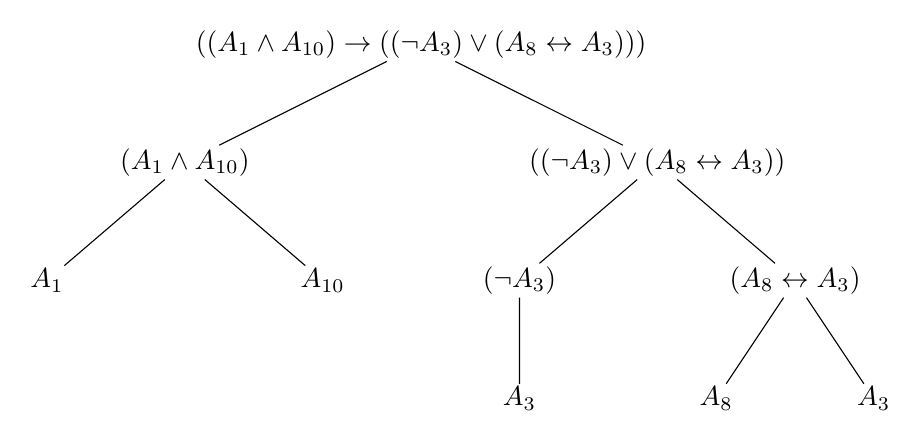
\begin{tikzpicture}[
  level distance=1.5cm,
  level 1/.style={sibling distance=6cm},
  level 2/.style={sibling distance=3.5cm},
  level 3/.style={sibling distance=2cm},
  every node/.style={inner sep=1pt}
]
\node {$((A_1 \wedge A_{10}) \to ((\neg A_3) \vee (A_8 \leftrightarrow A_3)))$}
  child { node {$(A_1 \wedge A_{10})$}
    child { node {$A_1$} }
    child { node {$A_{10}$} }
  }
  child { node {$((\neg A_3) \vee (A_8 \leftrightarrow A_3))$}
    child { node {$(\neg A_3)$}
      child { node {$A_3$} }
    }
    child { node {$(A_8 \leftrightarrow A_3)$}
      child { node {$A_8$} }
      child { node {$A_3$} }
    }
  };
\end{tikzpicture}


\begin{remark}[Building by closing under operations]\label{rem:closure-construction}
This sort of construction---taking some basic building blocks (here the
sentence symbols) and “closing” under some operations (here the five
formula-building operations)---occurs frequently both in logic and in other
branches of mathematics.
In Section~1.4, we will examine this kind of construction in a more general
setting.
\end{remark}

\begin{definition}[Construction sequence]\label{def:construction-sequence}
A \emph{construction sequence} is a finite sequence
$\langle \varepsilon_1,\dots,\varepsilon_n\rangle$ of expressions such that
for each $i\le n$ at least one of the following holds:
\begin{itemize}
  \item $\varepsilon_i$ is a sentence symbol;
  \item $\varepsilon_i = \mathcal{E}_{\neg}(\varepsilon_j)$ for some $j<i$;
  \item $\varepsilon_i = \mathcal{E}_{\square}(\varepsilon_j,\varepsilon_k)$
        for some $j<i$, $k<i$, where $\square$ is one of
        $\wedge,\vee,\rightarrow,\leftrightarrow$.
\end{itemize}
An expression $\alpha$ is a wff iff it appears as the last term of some
construction sequence.  We may think of $\varepsilon_i$ as the expression
produced at stage $i$ of the building process.
\end{definition}

\begin{remark}[From trees to sequences]
The construction sequence for our complex example above is obtained by
“flattening” its ancestral tree into a linear order: lower nodes come
earlier, higher nodes later.
\end{remark}

\begin{definition}[Closure under an operation]\label{def:closure}
A set $S$ is \emph{closed} under a one-place function $f$ if $x\in S$
implies $f(x)\in S$, and closed under a two-place function $g$ if
$x,y\in S$ imply $g(x,y)\in S$.
We say $S$ is closed under the five formula-building operations when
this holds for each of them.
\end{definition}

\begin{proposition}[Induction principle on wffs]\label{prop:induction}
Let $S$ be a set of wffs that contains all sentence symbols and is closed
under all five formula-building operations. Then $S$ is the set of \emph{all}
wffs.
\end{proposition}

\begin{remark}[Method 1.1.1: Proof by structural induction]\label{rem:struct-induction}
To prove a statement about all wffs, it suffices to:
\begin{itemize}
  \item verify it for all sentence symbols, and
  \item show that if it holds for $\alpha$ (and for $\beta$ when relevant),
        then it also holds for each of
        $(\neg \alpha)$,
        $(\alpha \wedge \beta)$,
        $(\alpha \vee \beta)$,
        $(\alpha \rightarrow \beta)$,
        $(\alpha \leftrightarrow \beta)$.
\end{itemize}
This is just an application of Proposition~\ref{prop:induction}.
\end{remark}

\begin{proof}[Proof of Proposition~\ref{prop:induction} (tree version)]
Take any wff $\alpha$.  It is built from sentence symbols by finitely many
applications of the formula-building operations; this is recorded in its
ancestral tree.  Starting from the leaves (sentence symbols in $S$) and
moving upward, closure of $S$ under each operation shows that every node
of the tree lies in $S$.  In particular, the root $\alpha$ lies in $S$.
\end{proof}

\begin{proof}[Second proof of Proposition~\ref{prop:induction} (sequence version)]
Let $\alpha$ be any wff.  Then $\alpha$ is the last term of some
construction sequence
$\langle\varepsilon_1,\dots,\varepsilon_n\rangle$.
Use strong numerical induction on $i$ to show that $\varepsilon_i\in S$
for all $i\le n$.
The induction step checks that whenever all earlier terms are in $S$, the
rules defining construction sequences plus the closure of $S$ under the
operations guarantee that $\varepsilon_i\in S$.
Hence $\alpha\in S$.
\end{proof}

\begin{example}[Balanced parentheses]\label{ex:balanced}
\emph{Claim.} Any expression with more left parentheses than right
parentheses is not a wff.

\emph{Idea.} Start from sentence symbols (no parentheses) and observe that
each formula-building operation adds parentheses only in matched pairs.
So wffs always have equally many left and right parentheses.

Formally, let $S$ be the set of expressions with equal numbers of left and
right parentheses.  Then:
\begin{itemize}
  \item all sentence symbols lie in $S$;
  \item each formula-building operation preserves membership in $S$.
\end{itemize}
By Proposition~\ref{prop:induction}, all wffs lie in $S$, so any expression
with unequal numbers of left and right parentheses cannot be a wff.
\end{example}

\begin{remark}[Formulas only grow]
Each operation $\mathcal{E}_{\square}(\alpha,\beta)$ produces an expression
that contains $\alpha$ (and $\beta$) as contiguous segments, plus extra
symbols; in particular, the result is longer than either input.
Thus every building step strictly increases length.

A useful consequence: if a wff $\varphi$ does not contain the symbol
$\mathbf{A}_4$, then no construction sequence for $\varphi$ ever needs to
use $\mathbf{A}_4$.
(See Exercise~\ref{ex:A4}.)
\end{remark}

%%%%%%%%%%%%%%%%%%%%%%%%%%%%%%%%%%%%%%%%%%%%%%%%%%%%
\section*{Exercises}
%%%%%%%%%%%%%%%%%%%%%%%%%%%%%%%%%%%%%%%%%%%%%%%%%%%%

\begin{exercise}[Exo 1.1]
Give three English sentences together with translations into our formal
language.  Choose sentences with interesting logical structure, and make
each translation contain at least 15 symbols.
\end{exercise}

\begin{exercise}[Exo 1.2]
Show that there are no wffs of length $2$, $3$, or $6$, but that any other
positive length occurs.
\end{exercise}

\begin{exercise}[Exo 1.3]
Let $\alpha$ be a wff.  Let $c$ be the number of occurrences of binary
connective symbols ($\wedge,\vee,\rightarrow,\leftrightarrow$) in $\alpha$,
and let $s$ be the number of occurrences of sentence symbols in $\alpha$.
For example, if $\alpha$ is $(\mathbf{A} \rightarrow (\neg \mathbf{A}))$
then $c=1$ and $s=2$.
Use Proposition~\ref{prop:induction} (structural induction) to show that $s = c+1$.
\end{exercise}

\begin{exercise}[Exo 1.4]\label{ex:A4}
Suppose we have a construction sequence ending in a wff $\varphi$ and that
$\varphi$ does not contain the symbol $\mathbf{A}_4$.
If we delete from the sequence all expressions that contain $\mathbf{A}_4$,
show that what remains is still a legal construction sequence.
\end{exercise}

\begin{exercise}[Exo 1.5]
Let $\alpha$ be a wff that does not contain the negation symbol $\neg$.
\begin{enumerate}
  \item[(a)] Show that the length of $\alpha$ (number of symbols) is odd.
  \item[(b)] Show that more than a quarter of the symbols of $\alpha$
             are sentence symbols.
\end{enumerate}
\emph{Hint.} Use structural induction to show that the length of $\alpha$
is of the form $4k+1$ and the number of sentence symbols is $k+1$ for some
integer $k$.
\end{exercise}

\end{document}
